\documentclass[aspectratio=169]{beamer}
\usetheme{Madrid}

\usepackage[utf8]{inputenc}
\usepackage[T1]{fontenc}
\usepackage{tikz}
\usetikzlibrary{arrows.meta,positioning,shapes.geometric}
\usepackage{xcolor}
\usepackage{listings}
\usepackage{booktabs}
\usepackage{colortbl}
\usepackage{array}

% ---------------- COULEURS PREFIXEES ----------------
\definecolor{cprimary}{HTML}{1B4F72}
\definecolor{caccent}{HTML}{2E86AB}
\definecolor{cdark}{HTML}{1A1A2E}
\definecolor{clight}{HTML}{F4F8FB}
\definecolor{cgreen}{HTML}{2D6A4F}
\definecolor{corange}{HTML}{E76F51}
\definecolor{cgray}{HTML}{6C757D}
\definecolor{cyellow}{HTML}{F4A261}

% ---------------- BEAMER STYLE ----------------
\setbeamercolor{structure}{fg=cprimary}
\setbeamercolor{background canvas}{bg=clight}
\setbeamercolor{frametitle}{bg=cprimary,fg=white}
\setbeamercolor{block title}{bg=caccent,fg=white}
\setbeamercolor{block body}{bg=clight}
\setbeamertemplate{navigation symbols}{}
\setbeamertemplate{footline}[frame number]

% ---------------- LISTINGS ----------------
\lstdefinestyle{mycode}{
  basicstyle=\ttfamily\scriptsize,
  breaklines=true,
  frame=single,
  backgroundcolor=\color{cdark!8},
  keywordstyle=\color{cprimary}\bfseries,
  stringstyle=\color{cgreen},
  commentstyle=\color{cgray}\itshape,
  rulecolor=\color{cprimary!30},
  upquote=true,
  keepspaces=true,
  columns=flexible
}
\lstset{style=mycode}

% ---------------- TITRE ----------------
\title{\textbf{Bot Discord de recommandation de recettes}}
\subtitle{RAG -- PostgreSQL/pgvector -- LLM local -- Discord.py}
\author{Elazar COHEN}
\date{Soutenance L3 Informatique}

\begin{document}

% ---- 1. TITRE ----
\begin{frame}
\titlepage
\end{frame}

% ---- 2. PLAN ----
\begin{frame}{Plan de la pr\'esentation}
\tableofcontents
\end{frame}

\section{Introduction}
\section{Architecture technique}
\section{Probl\`eme de performance}
\section{Organisation du travail}
\section{Bilan et am\'eliorations}

% ============================================================
% PARTIE 1 -- INTRODUCTION
% ============================================================

\begin{frame}{Contexte et motivation}
\begin{columns}[T]
\begin{column}{0.55\textwidth}
  \textbf{L'id\'ee de d\'epart}

  \vspace{0.3cm}
  Aider les gens \`a cuisiner \textbf{en fonction de leur budget}.

  \vspace{0.4cm}
  \begin{block}{\'Evolution du projet}
    \textbf{Application mobile} $\rightarrow$ hors comp\'etences fac, d\'ej\`a r\'ealis\'e

    \smallskip
    $\downarrow$

    \smallskip
    \textbf{Bot de groupe Discord} : communaut\'e, r\'eponse instantan\'ee
  \end{block}
\end{column}
\begin{column}{0.4\textwidth}
  \begin{center}
  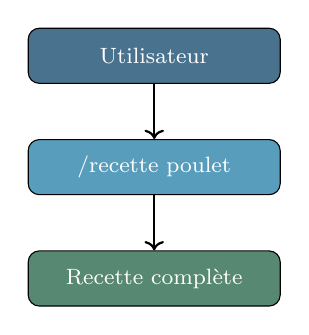
\begin{tikzpicture}[node distance=0.7cm, every node/.style={
      draw, rounded corners=4pt,
      minimum width=3.2cm, minimum height=0.7cm,
      font=\footnotesize, text centered}]
    \node[fill=cprimary!80, text=white] (u) {Utilisateur};
    \node[fill=caccent!80, text=white, below=of u] (b) {/recette poulet};
    \node[fill=cgreen!80, text=white, below=of b] (r) {Recette compl\`ete};
    \draw[->,thick] (u) -- (b);
    \draw[->,thick] (b) -- (r);
  \end{tikzpicture}
  \end{center}
\end{column}
\end{columns}

\vspace{0.3cm}
\textcolor{cgray}{\footnotesize Choix de Discord : facile \`a botter, exp\'erience naturelle de groupe}
\end{frame}

% ---- Objectifs techniques ----
\begin{frame}{Choix techniques}
\begin{columns}[T]
\begin{column}{0.32\textwidth}
  \begin{exampleblock}{Base de donn\'ees}
    \footnotesize
    PostgreSQL avec extension pgvector pour la recherche vectorielle
  \end{exampleblock}
\end{column}
\begin{column}{0.32\textwidth}
  \begin{exampleblock}{LLM local}
    \footnotesize
    Mistral via Ollama. Pas d'API payante. Contr\^ole total sur le syst\`eme
  \end{exampleblock}
\end{column}
\begin{column}{0.32\textwidth}
  \begin{exampleblock}{Bot Discord}
    \footnotesize
    discord.py. Commande /recette. R\'eponse async structur\'ee
  \end{exampleblock}
\end{column}
\end{columns}

\vspace{0.5cm}
\begin{center}
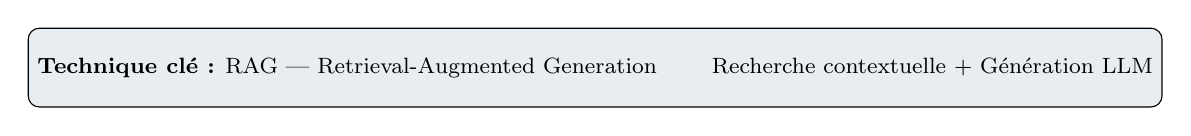
\begin{tikzpicture}
  \node[draw, rounded corners=4pt, fill=cprimary!10, minimum width=11cm, minimum height=1cm, font=\footnotesize] {
    \textbf{Technique cl\'e :} RAG --- Retrieval-Augmented Generation \hspace{0.5cm} Recherche contextuelle + G\'en\'eration LLM
  };
\end{tikzpicture}
\end{center}
\end{frame}

% ============================================================
% PARTIE 2 -- ARCHITECTURE
% ============================================================

\begin{frame}{Architecture globale --- pipeline complet}
\centering
\resizebox{\textwidth}{!}{%
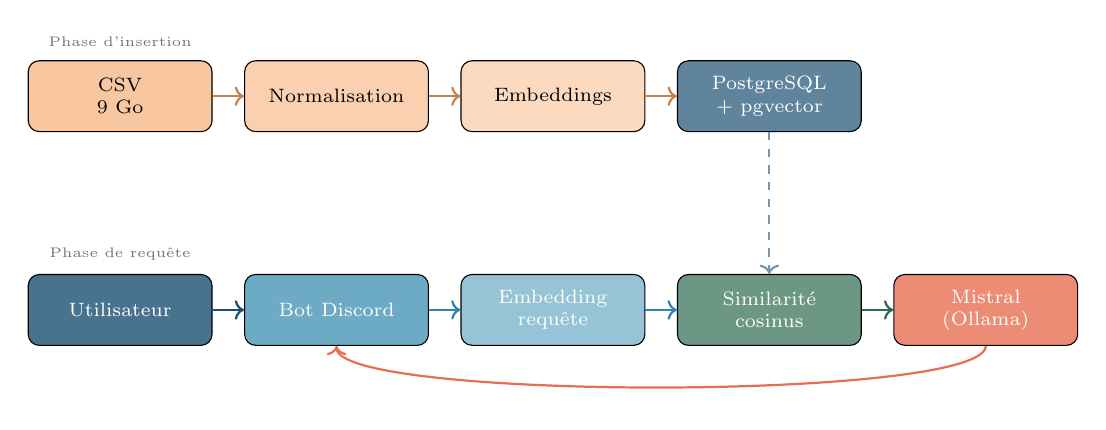
\begin{tikzpicture}[
  node distance=0.3cm and 0.4cm,
  box/.style={draw, rounded corners=4pt, minimum width=2.3cm,
              text width=2.1cm, minimum height=0.9cm,
              font=\scriptsize, align=center}
]
\node[box, fill=cyellow!60] (csv)  {CSV\\9 Go};
\node[box, fill=cyellow!50, right=of csv] (norm) {Normalisation};
\node[box, fill=cyellow!40, right=of norm] (emb)  {Embeddings};
\node[box, fill=cprimary!70, text=white, right=of emb] (pg) {PostgreSQL\\+ pgvector};

\node[box, fill=cprimary!80, text=white, below=1.8cm of csv] (user) {Utilisateur};
\node[box, fill=caccent!70, text=white, right=of user] (bot)  {Bot Discord};
\node[box, fill=caccent!50, text=white, right=of bot] (qemb) {Embedding\\requ\^ete};
\node[box, fill=cgreen!70, text=white, right=of qemb] (sim)  {Similarit\'e\\cosinus};
\node[box, fill=corange!80, text=white, right=of sim] (llm)  {Mistral\\(Ollama)};

\draw[->, thick, color=cyellow!80!black] (csv) -- (norm);
\draw[->, thick, color=cyellow!80!black] (norm) -- (emb);
\draw[->, thick, color=cyellow!80!black] (emb) -- (pg);
\draw[->, thick, color=cprimary] (user) -- (bot);
\draw[->, thick, color=caccent]  (bot) -- (qemb);
\draw[->, thick, color=caccent]  (qemb) -- (sim);
\draw[->, thick, color=cgreen]   (sim) -- (llm);
\draw[->, thick, dashed, color=cprimary!60] (pg) -- (sim);
\draw[->, thick, color=corange]  (llm.south) .. controls +(0,-0.7) and +(0,-0.7) .. (bot.south);

\node[font=\tiny, text=cgray, above=0.05cm of csv] {Phase d'insertion};
\node[font=\tiny, text=cgray, above=0.05cm of user] {Phase de requ\^ete};
\end{tikzpicture}%
}
\end{frame}


% ---- Schema BDD ----
\begin{frame}{Mod\`ele de donn\'ees}
\begin{columns}[T]
\begin{column}{0.52\textwidth}
\resizebox{\linewidth}{!}{%
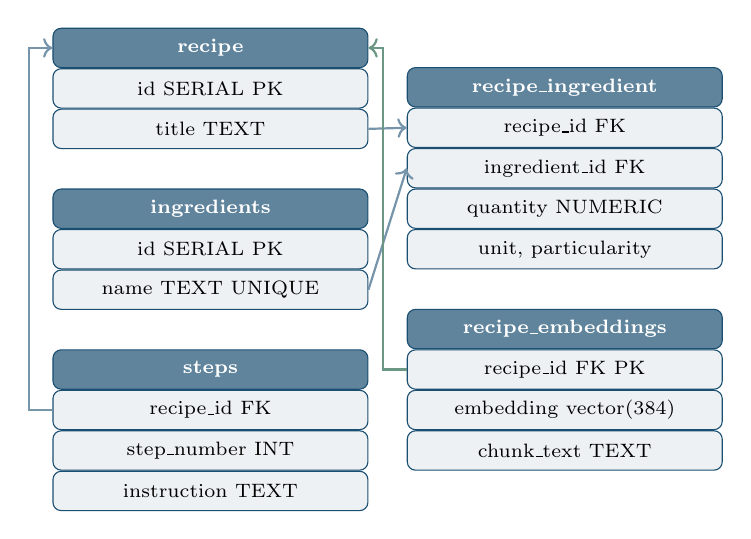
\begin{tikzpicture}[
  tab/.style={draw=cprimary, rounded corners=3pt, fill=cprimary!8,
              minimum width=4cm, minimum height=0.5cm, font=\scriptsize},
  head/.style={draw=cprimary, rounded corners=3pt, fill=cprimary!70,
               text=white, minimum width=4cm, minimum height=0.5cm,
               font=\scriptsize\bfseries}
]
  \node[head] (rt) at (0,0) {recipe};
  \node[tab, below=0cm of rt] (r1) {id SERIAL PK};
  \node[tab, below=0cm of r1] (r2) {title TEXT};

  \node[head, below=0.5cm of r2] (it) {ingredients};
  \node[tab, below=0cm of it] (i1) {id SERIAL PK};
  \node[tab, below=0cm of i1] (i2) {name TEXT UNIQUE};

  \node[head, below=0.5cm of i2] (st) {steps};
  \node[tab, below=0cm of st] (s1) {recipe\_id FK};
  \node[tab, below=0cm of s1] (s2) {step\_number INT};
  \node[tab, below=0cm of s2] (s3) {instruction TEXT};

  \node[head] (rit) at (4.5,-0.5) {recipe\_ingredient};
  \node[tab, below=0cm of rit] (ri1) {recipe\_id FK};
  \node[tab, below=0cm of ri1] (ri2) {ingredient\_id FK};
  \node[tab, below=0cm of ri2] (ri3) {quantity NUMERIC};
  \node[tab, below=0cm of ri3] (ri4) {unit, particularity};

  \node[head, below=0.5cm of ri4] (et) {recipe\_embeddings};
  \node[tab, below=0cm of et] (e1) {recipe\_id FK PK};
  \node[tab, below=0cm of e1] (e2) {embedding vector(384)};
  \node[tab, below=0cm of e2] (e3) {chunk\_text TEXT};

  \draw[->, thick, color=cprimary!60] (r2.east) -- (ri1.west);
  \draw[->, thick, color=cprimary!60] (i2.east) -- (ri2.west);
  \draw[->, thick, color=cprimary!60] (s1.west) -- ++(-0.3,0) |- (rt.west);
  \draw[->, thick, color=cgreen!70]   (e1.west) -- ++(-0.3,0) |- (rt.east);
\end{tikzpicture}%
}
\end{column}
\begin{column}{0.44\textwidth}
  \textbf{Points cl\'es :}
  \vspace{0.3cm}
  \begin{itemize}\footnotesize
    \item[\textcolor{cprimary}{\textbullet}] 5 tables 
    \item[\textcolor{cprimary}{\textbullet}] Ingr\'edients d\'edupliqu\'es (UNIQUE)
    \item[\textcolor{cgreen}{\textbullet}] \texttt{vector(384)} = all-MiniLM-L6-v2
    \item[\textcolor{corange}{\textbullet}] \texttt{chunk\_text} = texte complet pour le LLM
  \end{itemize}
  \vspace{0.4cm}
  \begin{block}{\scriptsize Requ\^ete de recherche}
  \vspace{0.1cm}
  {\ttfamily\tiny
  SELECT recipe\_id,\\
  \quad 1 - (embedding <=> query)\\
  FROM recipe\_embeddings\\
  ORDER BY embedding <=> query\\
  LIMIT 5;
  }
  \end{block}
\end{column}
\end{columns}
\end{frame}

% ============================================================
% PARTIE 3 -- PERFORMANCE
% ============================================================

\begin{frame}{Probl\`eme de performance --- \'etat initial}
\begin{columns}[T]
\begin{column}{0.5\textwidth}
  \begin{center}
  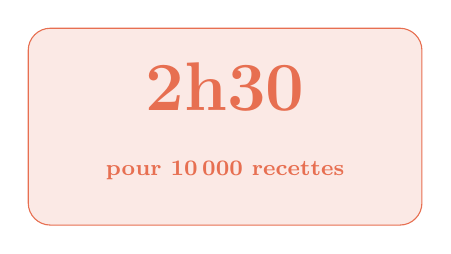
\begin{tikzpicture}
    \node[draw=corange, fill=corange!15, rounded corners=8pt,
          minimum width=5cm, minimum height=2.5cm,
          font=\Large\bfseries, text=corange] {
      \begin{tabular}{c}
        \Huge\textbf{2h30}\\[0.2cm]
        \footnotesize pour 10\,000 recettes
      \end{tabular}
    };
  \end{tikzpicture}
  \end{center}
  \vspace{0.3cm}
  \textcolor{cgray}{\footnotesize
    Dataset complet : $\approx$ 2 millions de recettes.
    Estimation : \textbf{plusieurs semaines}
  }
\end{column}
\begin{column}{0.46\textwidth}
  \textbf{Code initial :}
  \vspace{0.2cm}
  \begin{itemize}\footnotesize
    \item[\textcolor{corange}{\textbullet}] 1 connexion ouverte par recette
    \item[\textcolor{corange}{\textbullet}] 1 INSERT par ligne, par table
    \item[\textcolor{corange}{\textbullet}] Embedding calcul\'e recette par recette
    \item[\textcolor{corange}{\textbullet}] Des \textbf{dizaines de milliers} d'aller-retours avec la BDD
  \end{itemize}
  \vspace{0.3cm}
  \begin{block}{\scriptsize Probl\`eme (pseudo-code)}
  \vspace{0.05cm}
  {\ttfamily\scriptsize
  for recipe in dataset:\\
  \quad emb = model.encode(recipe)\\
  \quad conn = db.connect()\\
  \quad cur.execute("INSERT ...")
  }
  \end{block}
\end{column}
\end{columns}
\end{frame}

% ---- Les deux goulots ----
\begin{frame}{Deux goulots d'\'etranglement identifi\'es}
\begin{columns}[T]
\begin{column}{0.48\textwidth}
  \begin{alertblock}{Goulot \#1 --- Transactions}
  \footnotesize
  Ouvrir une connexion + transaction pour chaque recette = overhead \'enorme.

  \smallskip
  PostgreSQL doit valider (COMMIT) \`a chaque fois. 10\,000 recettes x 5 tables = \textbf{50\,000+ requ\^etes}.

  \smallskip
  \textbf{Solution :} une seule transaction globale + COPY PostgreSQL
  \end{alertblock}
\end{column}
\begin{column}{0.48\textwidth}
  \begin{alertblock}{Goulot \#2 --- Embeddings (90--95\% du temps)}
  \footnotesize
  \texttt{model.encode()} sur une recette \`a la fois = tr\`es inefficace.

  \smallskip
  SentenceTransformer est optimis\'e pour les \textbf{lots (batches)}. 1 \`a la fois = pas de vectorisation CPU.

  \smallskip
  \textbf{Solution :} \texttt{model.encode(chunks, batch\_size=1024)}
  \end{alertblock}
\end{column}
\end{columns}
\end{frame}



% ---- Tableau comparatif ----
\begin{frame}{R\'esultats --- comparaison des performances}
\begin{center}
\renewcommand{\arraystretch}{1.4}
\begin{tabular}{lccl}
\toprule
\textbf{Etape} & \textbf{Temps} & \textbf{Gain} & \textbf{Changement} \\
\midrule
\rowcolor{corange!20}
Etat initial & 2h30 & --- & INSERT un par un, encode un par un \\
\rowcolor{cyellow!30}
Batch embeddings & $\approx$10 min & $\times$15 & \texttt{batch\_size=1024} \\
\rowcolor{cgreen!20}
+ COPY PostgreSQL & 3--5 min & $\times$50 & CSV en memoire, 1 transaction \\
\midrule
\rowcolor{cprimary!10}
Insertion BDD seule & <1 sec & --- & Quelques millisecondes \\
Embeddings seuls & 3--5 min & --- & 90--95\% du temps total \\
\bottomrule
\end{tabular}
\end{center}

\vspace{0.4cm}
\begin{block}{Limite restante}
\footnotesize
Les embeddings sur \textbf{CPU} restent le vrai goulot. Sur GPU, le gain serait de x10 a x50 supplementaires --- mais les machines de la fac n'ont pas pgvector installe.
\end{block}
\end{frame}

% ============================================================
% PARTIE 4 -- ORGANISATION
% ============================================================

\begin{frame}{Organisation du travail --- 3 grandes phases}
\begin{center}
  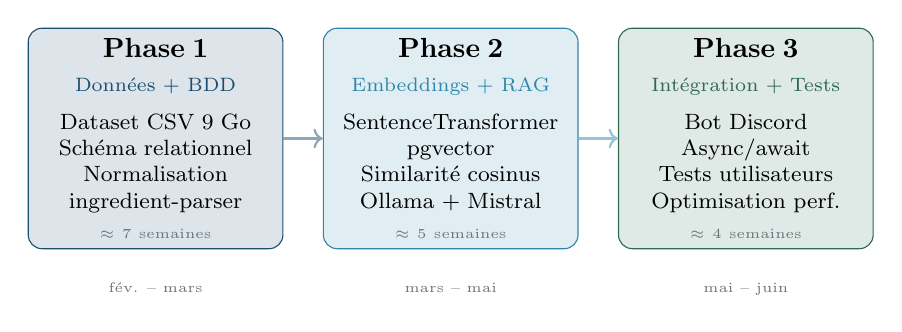
\begin{tikzpicture}[
  phase/.style={draw, rounded corners=5pt, minimum width=3.2cm,
                minimum height=2.8cm, font=\scriptsize, text centered,
                text width=3cm},
  node distance=0.5cm
]
\node[phase, fill=cprimary!15, draw=cprimary] (p1) {
  \textbf{\normalsize Phase 1}\par
  \vspace{0.15cm}
  \textcolor{cprimary}{Donn\'ees + BDD}\par
  \vspace{0.15cm}
  \footnotesize
  Dataset CSV 9 Go\par
  Sch\'ema relationnel\par
  Normalisation\par
  ingredient-parser\par
  \vspace{0.1cm}
  \textcolor{cgray}{\tiny $\approx$ 7 semaines}
};
\node[phase, fill=caccent!15, draw=caccent, right=0.5cm of p1] (p2) {
  \textbf{\normalsize Phase 2}\par
  \vspace{0.15cm}
  \textcolor{caccent}{Embeddings + RAG}\par
  \vspace{0.15cm}
  \footnotesize
  SentenceTransformer\par
  pgvector\par
  Similarit\'e cosinus\par
  Ollama + Mistral\par
  \vspace{0.1cm}
  \textcolor{cgray}{\tiny $\approx$ 5 semaines}
};

\node[phase, fill=cgreen!15, draw=cgreen, right=0.5cm of p2] (p3) {
  \textbf{\normalsize Phase 3}\par
  \vspace{0.15cm}
  \textcolor{cgreen}{Int\'egration + Tests}\par
  \vspace{0.15cm}
  \footnotesize
  Bot Discord\par
  Async/await\par
  Tests utilisateurs\par
  Optimisation perf.\par
  \vspace{0.1cm}
  \textcolor{cgray}{\tiny $\approx$ 4 semaines}
};

\draw[->,thick,color=cprimary!50] (p1.east) -- (p2.west);
\draw[->,thick,color=caccent!50]  (p2.east) -- (p3.west);

\node[font=\tiny, text=cgray, below=0.3cm of p1] {f\'ev. -- mars};
\node[font=\tiny, text=cgray, below=0.3cm of p2] {mars -- mai};
\node[font=\tiny, text=cgray, below=0.3cm of p3] {mai -- juin};
\end{tikzpicture}

\end{center}
\vspace{0.2cm}
\begin{columns}
\begin{column}{0.48\textwidth}
\begin{exampleblock}{\scriptsize D\'efi de la normalisation}
\footnotesize
Donn\'ees en anglais, unit\'es am\'ericaines (cups, oz). Utilisation de \texttt{ingredient-parser} pour extraire nom, quantit\'e, unit\'e.
\end{exampleblock}
\end{column}
\begin{column}{0.48\textwidth}
\begin{exampleblock}{\scriptsize Tests utilisateurs}
\footnotesize
Bot lanc\'e dans un serveur Discord priv\'e. Retours sur la qualit\'e des recettes. Am\'elioration du prompt syst\`eme.
\end{exampleblock}
\end{column}
\end{columns}
\end{frame}

% ============================================================
% PARTIE 5 -- BILAN
% ============================================================

\begin{frame}{Bilan --- forces et limites}
\begin{columns}[T]
\begin{column}{0.48\textwidth}
  \begin{exampleblock}{Ce qui fonctionne}
  \footnotesize
  \begin{itemize}
    \item Bot utilisable en conditions r\'eelles
    \item RAG efficace sur des requ\^etes vagues
    \item 10\,000 recettes ins\'er\'ees en 3--5 min
    \item Pipeline complet autonome (LLM local)
    \item Prompt structur\'e : recette coh\'erente
  \end{itemize}
  \end{exampleblock}
\end{column}
\begin{column}{0.48\textwidth}
  \begin{alertblock}{Limites identifi\'ees}
  \footnotesize
  \begin{itemize}
    \item Mistral local moins puissant qu'un LLM cloud
    \item Qualit\'e d\'ependante du dataset
    \item Embeddings sur CPU : goulot restant
    \item Pas de filtre allergies / r\'egime
  \end{itemize}
  \end{alertblock}
\end{column}
\end{columns}
\end{frame}

\begin{frame}{Am\'eliorations possibles}
\begin{columns}[T]
\begin{column}{0.48\textwidth}
  \textbf{Performance}
  \vspace{0.2cm}
  \begin{itemize}\footnotesize
    \item[\textcolor{cprimary}{\textbf{1.}}] \textbf{Embeddings sur GPU} : x10 a x50 plus rapide, dataset complet en quelques minutes
  \end{itemize}
\end{column}
\begin{column}{0.48\textwidth}
  \textbf{Fonctionnalit\'es}
  \vspace{0.2cm}
  \begin{itemize}\footnotesize
    \item[\textcolor{cgreen}{\textbf{2.}}] \textbf{Filtrage nutritionnel} : recherche vectorielle + filtres SQL (budget, allergies, r\'egime)
    \item[\textcolor{cgreen}{\textbf{3.}}] \textbf{LLM plus puissant} : API cloud pour la g\'en\'eration, recherche vectorielle en local
  \end{itemize}
\end{column}
\end{columns}

\vspace{0.5cm}
\begin{center}

\begin{tikzpicture}
  \node[draw=cprimary, rounded corners=5pt, fill=cprimary!8, minimum width=11cm,
        minimum height=0.9cm, font=\small] {
    \textbf{Ce projet est extensible :} BDD, embeddings et LLM sont des briques ind\'ependantes.
  };
\end{tikzpicture}
\end{center}
\end{frame}



\begin{frame}{Exemple d'utilisation du bot}
\begin{columns}[T]
\begin{column}{0.5\textwidth}
    \centering
    
\includegraphics[width=\linewidth]{cookingBotProfil.png}

    \vspace{0.2cm}
    \footnotesize\textcolor{cgray}{Profil Discord du bot}
  \end{column}
  \begin{column}{0.5\textwidth}
    
  \end{column}
  \end{columns}
\end{frame}

\begin{frame}{Exemple d'utilisation du bot}
\begin{columns}[T]
\begin{column}{0.5\textwidth}
  \centering
  
\includegraphics[width=\linewidth]{cookingBotProfil.png}

  \vspace{0.2cm}
  \footnotesize\textcolor{cgray}{Profil Discord du bot}
\end{column}
\begin{column}{0.5\textwidth}
  \centering
  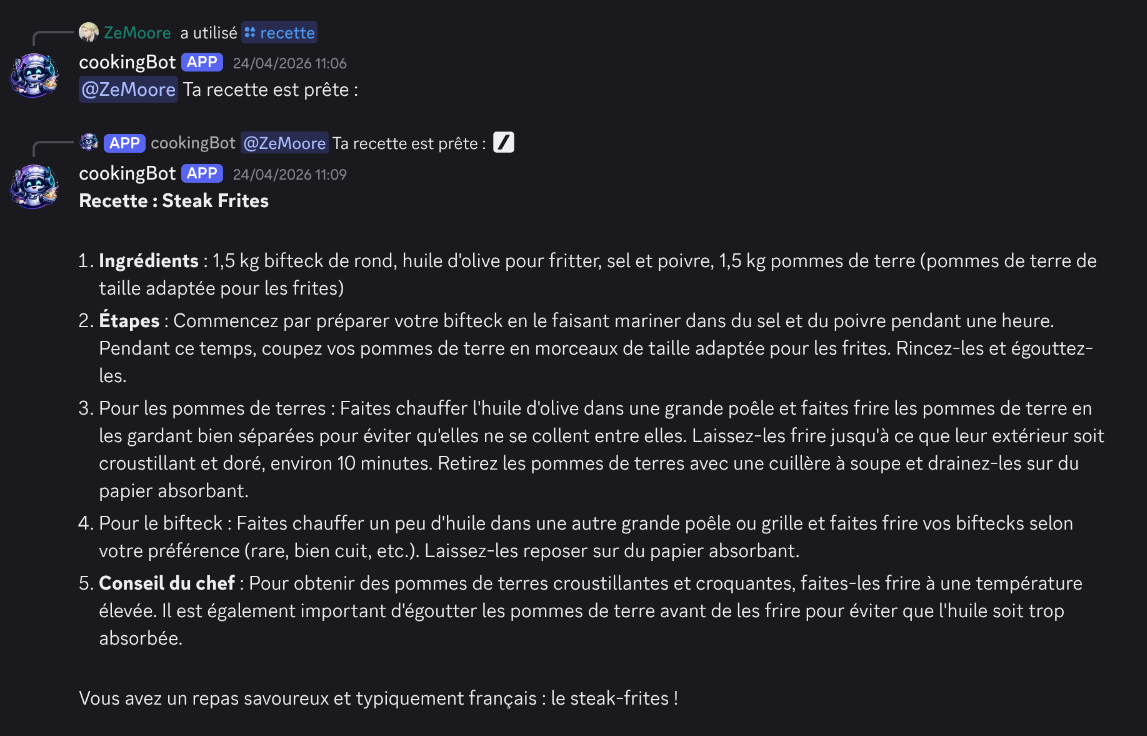
\includegraphics[width=\linewidth]{exemple_recette.png}

  \vspace{0.2cm}
  \footnotesize\textcolor{cgray}{Exemple de recette g\'en\'er\'ee via \texttt{/recette}}
\end{column}
\end{columns}
\end{frame}

% ---- Conclusion ----
\begin{frame}{Conclusion}
\begin{columns}[T]
\begin{column}{0.55\textwidth}
  \textbf{Ce que ce projet m'a appris :}
  \vspace{0.3cm}
  \begin{itemize}\footnotesize
    \item Construire un syst\`eme complet de bout en bout (donn\'ees $\rightarrow$ BDD $\rightarrow$ LLM $\rightarrow$ bot)
    \item Comprendre et impl\'ementer le \textbf{RAG}
    \item Diagnostiquer des probl\`emes de \textbf{performance r\'eels} (x50 de gain)
    \item Travailler avec des biblioth\`eques NLP (SentenceTransformer, ingredient-parser)
    \item D\'eveloppement async avec discord.py
  \end{itemize}
\end{column}
\begin{column}{0.4\textwidth}
  \begin{center}
  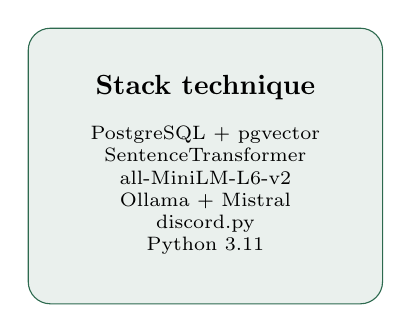
\begin{tikzpicture}
  \node[draw=cgreen, rounded corners=8pt, fill=cgreen!10,
        minimum width=4.5cm, minimum height=3.5cm,
        font=\scriptsize, text centered] {
    \begin{tabular}{c}
      \textbf{\normalsize Stack technique}\\[0.3cm]
      PostgreSQL + pgvector\\
      SentenceTransformer\\
      all-MiniLM-L6-v2\\
      Ollama + Mistral\\
      discord.py\\
      Python 3.11
    \end{tabular}
  };
  \end{tikzpicture}
  \end{center}
\end{column}
\end{columns}

\end{frame}

\begin{frame}{Questions}
  \vspace{0.6cm}
  \begin{center}
    \Large\textbf{Merci pour votre attention}

    \vspace{0.2cm}
    \normalsize\textcolor{cgray}{Questions ?}
  \end{center}
\end{frame}

\end{document}